\subsection{The box product}

In this section, we explore another application of the cross product.
Recall that we can use the cross product to find the the area of a
parallelogram. As we will now show, we can also use the cross product
together with the dot product to find the volume of a
parallelepiped. We begin with a definition.

\begin{definition}{Parallelepiped}{parallelepiped}
  The parallelepiped\index{parallelepiped} determined by three
  vectors $\vect{u}$, $\vect{v}$, and $\vect{w}$ consists of the set of
  points of the form
  \begin{equation*}
    r\/\vect{u}+s\/\vect{v}+t\/\vect{w},
  \end{equation*}
  where $r,s,t$ are real numbers between $0$ and $1$, inclusive. The
  parallelepiped is a $3$-dimensional body bounded by parallelograms
  as shown in this picture.
  \begin{center}
    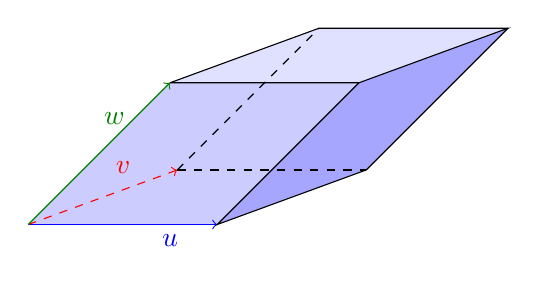
\begin{tikzpicture}[scale=1.2]
      \fill[blue!20] (0,0,0) -- (2,0,0) -- (3.5,1.5,0) -- (1.5,1.5,0) -- cycle;
      \fill[blue!35] (2,0,0) -- ++(1.5,1.5,0) -- ++(1,0,-1.5) -- ++(-1.5,-1.5,0) -- cycle;
      \fill[blue!12] (1.5,1.5,0) -- ++(2,0,0) -- ++(1,0,-1.5) -- ++(-2,0,0) -- cycle;
      \draw[blue,->](0,0,0) -- node [below, near end] {$\vect{u}$} (2,0,0); %% u
      \draw[red,dashed,->](0,0,0) -- node [above left, near end] {$\vect{v}$} (1,0,-1.5); %% v
      \draw[green!50!black,->](0,0,0) -- node [left, near end] {$\vect{w}$} (1.5,1.5,0); %% w
      \draw[dashed](1,0,-1.5)--(3,0,-1.5);
      \draw[dashed](1,0,-1.5)--(2.5,1.5,-1.5);
      \draw(1.5,1.5,0)--(3.5,1.5,0)--(4.5,1.5,-1.5)--(2.5,1.5,-1.5)--(1.5,1.5,0);
      \draw(3.5,1.5,0)--(2,0,0)--(3,0,-1.5)--(4.5,1.5,-1.5);
    \end{tikzpicture}
  \end{center}
\end{definition}

Notice that the base of the parallelepiped is the parallelogram
determined by the vectors $\vect{u}$ and $\vect{v}$. Therefore, its
area is equal to $\norm{\vect{u}\times\vect{v}}$. The height of the
parallelepiped is $\norm{\vect{w}}\cos\theta$, where $\theta$ is the
angle between $\vect{w}$ and $\vect{u}\times\vect{v}$, as shown in
this picture.
\begin{center}
  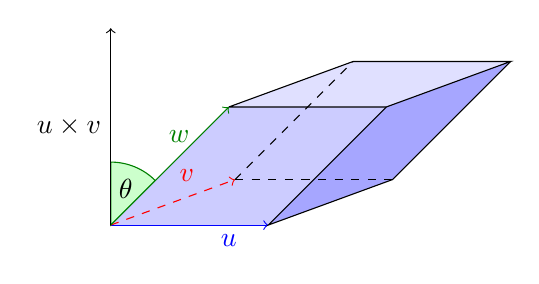
\begin{tikzpicture}[scale=1]
    \filldraw[fill=green!20,draw=green!50!black] (0,0) -- (45:8mm) arc (45:90:8mm) -- cycle;
    \fill[blue!20] (0,0,0) -- (2,0,0) -- (3.5,1.5,0) -- (1.5,1.5,0) -- cycle;
    \fill[blue!35] (2,0,0) -- ++(1.5,1.5,0) -- ++(1,0,-1.5) -- ++(-1.5,-1.5,0) -- cycle;
    \fill[blue!12] (1.5,1.5,0) -- ++(2,0,0) -- ++(1,0,-1.5) -- ++(-2,0,0) -- cycle;
    \draw[blue,->](0,0,0) -- node [below, near end] {$\vect{u}$} (2,0,0); %% u
    \draw[red,dashed,->](0,0,0) -- node [above left, near end] {$\vect{v}$} (1,0,-1.5); %% v
    \draw[green!50!black,->](0,0,0) -- node [left, near end] {$\vect{w}$} (1.5,1.5,0); %% w
    \draw[->](0,0,0) -- node[left] {$\vect{u}\times\vect{v}$} (0,2.5,0);
    \draw[dashed](1,0,-1.5)--(3,0,-1.5);
    \draw[dashed](1,0,-1.5)--(2.5,1.5,-1.5);
    \draw(1.5,1.5,0)--(3.5,1.5,0)--(4.5,1.5,-1.5)--(2.5,1.5,-1.5)--(1.5,1.5,0);
    \draw(3.5,1.5,0)--(2,0,0)--(3,0,-1.5)--(4.5,1.5,-1.5);
    \node at (67.5:5mm){$\theta$};
  \end{tikzpicture}
\end{center}
The volume of this parallelepiped is the area of the base times the
height which is just
\begin{equation*}
  \norm{\vect{u}\times \vect{v}} \norm{\vect{w}} \cos \theta =
  (\vect{u}\times\vect{v}) \dotprod \vect{w}.
\end{equation*}
This expression is known as the
\textbf{box product}\index{box product} and is sometimes written as
$\boxprod{\vect{u},\vect{v},\vect{w}}$.

Consider what happens if you interchange $\vect{v}$ with $\vect{w}$ or
$\vect{u}$ with $\vect{w}$.  Geometrically, we can see that this
merely introduces a minus sign. We find that the box product of three
vectors equals the volume of the parallelepiped determined by the
three vectors if the three vectors form a right-handed system, and the
negative of the volume if the vectors form a left-handed system.
We summarize this in the following proposition:

\begin{proposition}{The box product}{box-product}
  Let $\vect{u}, \vect{v}, \vect{w}$ be three vectors in $\R^n$ that
  define a parallelepiped. The box product
  $(\vect{u}\times\vect{v}) \dotprod \vect{w}$ is equal to:
  \begin{itemize}
  \item The volume%
    \index{box product!volume of parallelepiped}%
    \index{volume!of parallelepiped}%
    \index{parallelepiped!volume} of the parallelepiped, if
    $\vect{u}, \vect{v}, \vect{w}$ form a right-handed system.
  \item The negative of the volume of the parallelepiped, if
    $\vect{u}, \vect{v}, \vect{w}$ form a left-handed system.
  \end{itemize}
  In any case, the volume of the parallelepiped can be computed as the
  absolute value of the box product, given by
  $\abs{(\vect{u}\times\vect{v}) \dotprod \vect{w}}$.
\end{proposition}

\begin{example}{Volume of a parallelepiped}{parallelepiped-volume}
  Find the volume of the parallelepiped determined by the vectors
  \begin{equation*}
    \vect{u}
    =
    \begin{mymatrix}{r}
      1 \\
      2 \\
      -5
    \end{mymatrix}, \quad
    \vect{v}
    =
    \begin{mymatrix}{r}
      1 \\
      3 \\
      -6
    \end{mymatrix}, \quad
    \vect{w}
    =
    \begin{mymatrix}{r}
      3 \\
      2 \\
      3
    \end{mymatrix}.
  \end{equation*}
\end{example}

\begin{solution}
  According to the above discussion, we can take the cross product of
  any two of these vectors, and then the dot product with the third
  vector. The result will be either plus or minus the desired
  volume. Therefore we can obtain the volume by taking the absolute value.

  We first compute the cross product of $\vect{u}$ and $\vect{v}$:
  \begin{equation*}
    \vect{u} \times \vect{v}
    =
    \begin{mymatrix}{r}
      1 \\
      2 \\
      -5
    \end{mymatrix}
    \times
    \begin{mymatrix}{r}
      1 \\
      3 \\
      -6
    \end{mymatrix} \\
    =\begin{mymatrix}{c}
      (2)(-6) - (-5)(3) \\
      (-5)(1) - (1)(-6) \\
      (1)(3)  - (2)(1)  \\
    \end{mymatrix}
    =
    \begin{mymatrix}{r}
      3 \\
      1 \\
      1
    \end{mymatrix}
  \end{equation*}
  Then we take the dot product of this vector with $\vect{w}$:
  \begin{equation*}
    (\vect{u} \times \vect{v}) \dotprod \vect{w}
    =
    \begin{mymatrix}{r}
      3 \\
      1 \\
      1
    \end{mymatrix}
    \dotprod
    \begin{mymatrix}{r}
      3 \\
      2 \\
      3
    \end{mymatrix} \\
    = 9+2+3
    = 14.
  \end{equation*}
  Thus, the volume of the parallelepiped is 14 cubic units.
\end{solution}

The following is a consequence of Proposition~\ref{prop:box-product}:

\begin{corollary}{Right- and left-handed systems of vectors}{box-product-right-handed}
  The box product $(\vect{u}\times\vect{v}) \dotprod \vect{w}$ is:
  \begin{itemize}
  \item Positive, if $\vect{u},\vect{v},\vect{w}$ form a right-handed system.
  \item Negative, if $\vect{u},\vect{v},\vect{w}$ form a left-handed system.
  \item Zero, if $\vect{u},\vect{v},\vect{w}$ are coplanar.
  \end{itemize}
\end{corollary}

\begin{example}{Right- and left-handed systems of vectors}{box-product-right-handed}
  Which of the following systems of vectors
  $\vect{u},\vect{v},\vect{w}$ is right-handed? Which one is left-handed?
  Which one is coplanar?
  \begin{enumialphparenastyle}
    \begin{enumerate}
    \item $\vect{u}=\mat{1,2,0}^T$, $\vect{v}=\mat{0,0,1}^T$, $\vect{w}=\mat{1,-1,1}^T$.
    \item $\vect{u}=\mat{1,1,1}^T$, $\vect{v}=\mat{1,2,3}^T$, $\vect{w}=\mat{0,1,1}^T$.
    \item $\vect{u}=\mat{0,1,2}^T$, $\vect{v}=\mat{1,2,2}^T$, $\vect{w}=\mat{1,1,0}^T$.
    \end{enumerate}
  \end{enumialphparenastyle}
\end{example}

\begin{solution}
  \begin{enumialphparenastyle}
    \begin{enumerate}
    \item We have
      $\boxprod{\vect{u},\vect{v},\vect{w}} = (\vect{u}\times\vect{v})
      \dotprod \vect{w} = \mat{2,-1,0}^T\dotprod\mat{1,-1,1}^T=3$, so
      the box product is positive and the system of vectors
      $\vect{u},\vect{v},\vect{w}$ is right-handed.
    \item We have
      $\boxprod{\vect{u},\vect{v},\vect{w}} = (\vect{u}\times\vect{v})
      \dotprod \vect{w} = \mat{1,-2,1}^T\dotprod\mat{0,1,1}^T=-1$, so
      the box product is negative and the system is left-handed.
    \item We have
      $\boxprod{\vect{u},\vect{v},\vect{w}} = (\vect{u}\times\vect{v})
      \dotprod \vect{w} = \mat{-2,2,-1}^T\dotprod\mat{1,1,0}^T=0$, so
      the box product is zero and the vectors are coplanar.
    \end{enumerate}
  \end{enumialphparenastyle}
\end{solution}

We finish this section with a law involving the dot product and the
cross product. It represents a fundamental observation that comes
directly from the geometric definition of the box product.

\begin{proposition}{Box product law}{order-of-product}
  Let $\vect{u}$, $\vect{v}$, and $\vect{w}$ be vectors. Then
  $(\vect{u}\times\vect{v}) \dotprod \vect{w}=\vect{u}\dotprod
  (\vect{v}\times \vect{w})$.
\end{proposition}

\begin{proof}
  This follows from observing that both
  $(\vect{u}\times \vect{v}) \dotprod \vect{w}$ and
  $\vect{u}\dotprod (\vect{v}\times \vect{w})$ compute the same
  box product, i.e., they either both give the volume of the
  parallelepiped or they both give the negative of the volume.

  Alternatively, we can calculate each product explicitly:
  \begin{eqnarray*}
    (\vect{u}\times \vect{v}) \dotprod \vect{w}
    &=&
        u_2v_3w_1 - u_3v_2w_1
        + u_3v_1w_2 - u_1v_3w_2
        + u_1v_2w_3 - u_2v_1w_3, \\
    \vect{u}\dotprod (\vect{v}\times \vect{w})
    &=&
        u_2v_3w_1 - u_3v_2w_1
        + u_3v_1w_2 - u_1v_3w_2
        + u_1v_2w_3 - u_2v_1w_3.
  \end{eqnarray*}
  In Chapter~\ref{cha:determinants}, you will learn that these
  expressions are a special case of a determinant.
\end{proof}

